\section{Myoblast Segmentation using Stardist}
Typical instance segmentation methods also suffer from the suppresion of valid objects or the merging instances given overlapping instances. In order to better segment the myoblasts, a cell detection method called \texttt{StarDist} \cite{schmidt2018, weigert2020} is used. It was developed with the intent to segment microscopy data like the nuclei found in this project.

In brief, a convolutional neural network is trained to predict polygons imitating typical cell shapes for every pixel of the image. More concretely, it predicts a star-convex polygon for every (non-background) pixel. Intuitively speaking, a star-convex set $\mathcal{S}$ is one where there exists one point $s_{0}$ such that for every point $s \in \mathcal{S}$ the line segment connecting $s_{0}$ to $s$ is element of $\mathcal{S}$. For every pixel such a shape can be approximated by following $n$ predefined radial directions for a distance of $\{r^{k}_{ij}\}^{n}_{k = 1}$ starting from the pixel parametrized by $i,j$ serving as $s_{0}$. Furthermore \textcolor{red}{add $d_{ij}$, add reffig, add discussion of loss and weights}

\begin{figure}
	\centering
	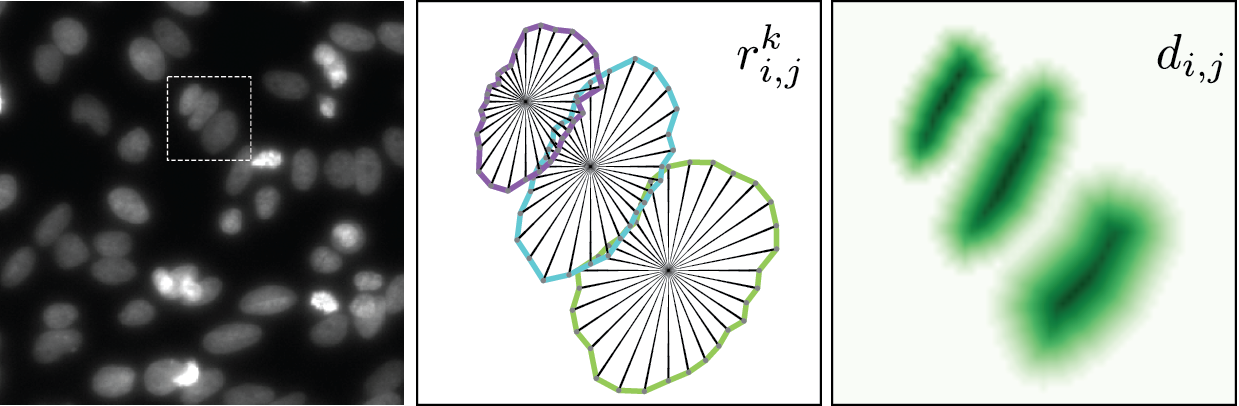
\includegraphics[width=\textwidth]{"images/star_convexity_explained.png"}
	\caption{Example of an area that is complicated to segment due to overlaps. \texttt{StarDist} creates the segementation by forming star-convex polygons and computing the probability to belong to said instance. Source: \Cite{schmidt2018}.}
	\label{figstardistexplained}
\end{figure}

In \texttt{StarDist}, the \texttt{U-Net} architecture \cite{RonnebergerFB15} is used as the backbone and is slightly modified by adding another 128-channel 3x3-convolutional layer with ReLu activation to the \texttt{U-Net} output. This output, in turn, is fed into two other convolutional layers. The first one is a single channel convolutional layer with sigmoid activation meant learn object probabilities. The second one has a linear activation and as many channels as there are radial directions.